% LaTeX Figure Snippets for Banquet Fine-Tuning Run 002

\begin{figure}[t]
    \centering
    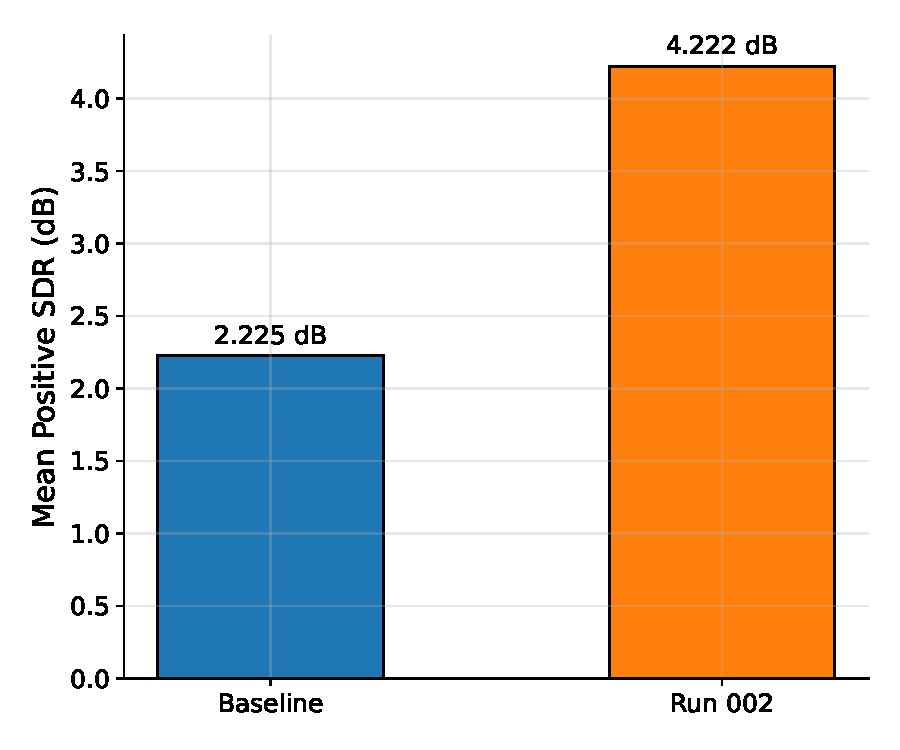
\includegraphics[width=0.8\linewidth]{paper_figures/run002_test_overall_sdr.pdf}
    \caption{Overall held-out TEST Source-to-Distortion Ratio (SDR) in decibels (dB), comparing the baseline model with the Run 002 fine-tuned model. Higher SDR indicates lower distortion. On the held-out TEST set, the fine-tuned model achieved higher mean positive SDR than the baseline.}
    \label{fig:test_overall_sdr}
\end{figure}

\begin{figure}[t]
    \centering
    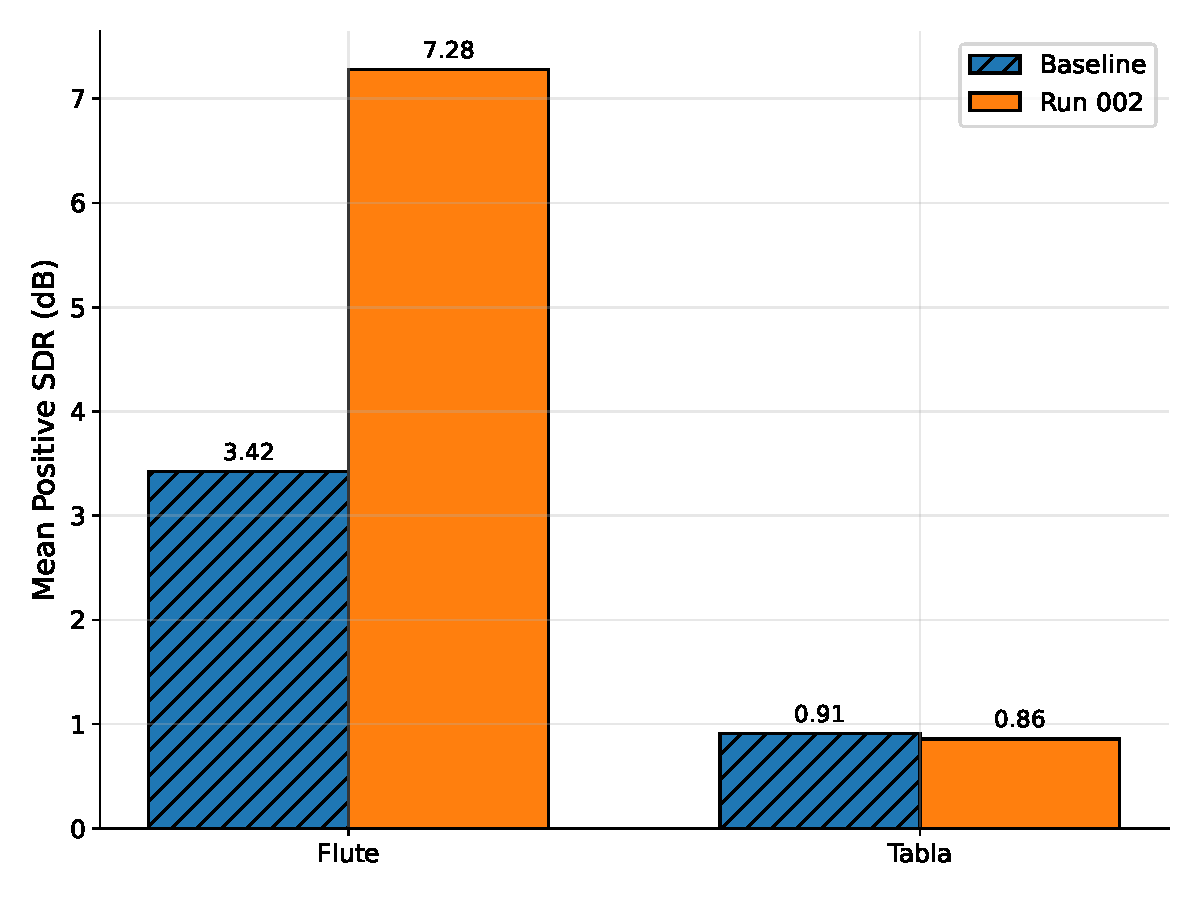
\includegraphics[width=0.8\linewidth]{paper_figures/run002_test_per_instrument_sdr.pdf}
    \caption{Per-instrument mean positive SDR on the held-out TEST set for instruments with valid positive TEST representations. Fine-tuning substantially improved Flute SDR, while Tabla SDR remained approximately comparable to the baseline.}
    \label{fig:test_per_instrument_sdr}
\end{figure}

\begin{figure}[t]
    \centering
    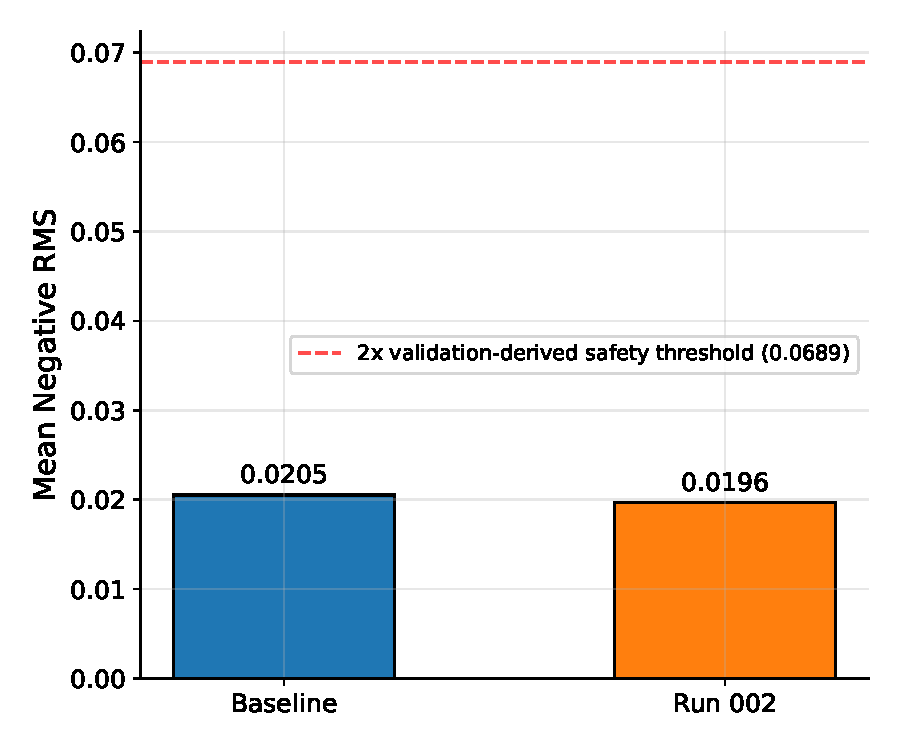
\includegraphics[width=0.8\linewidth]{paper_figures/run002_test_negative_rms.pdf}
    \caption{Mean negative-query RMS on the held-out TEST set, where lower values indicate lower output energy for queries corresponding to absent instruments. The dashed line denotes the $2\times$ safety threshold derived from the validation baseline and used during checkpoint selection; the TEST measurements shown here were obtained independently after model selection.}
    \label{fig:test_negative_rms}
\end{figure}

\begin{figure}[t]
    \centering
    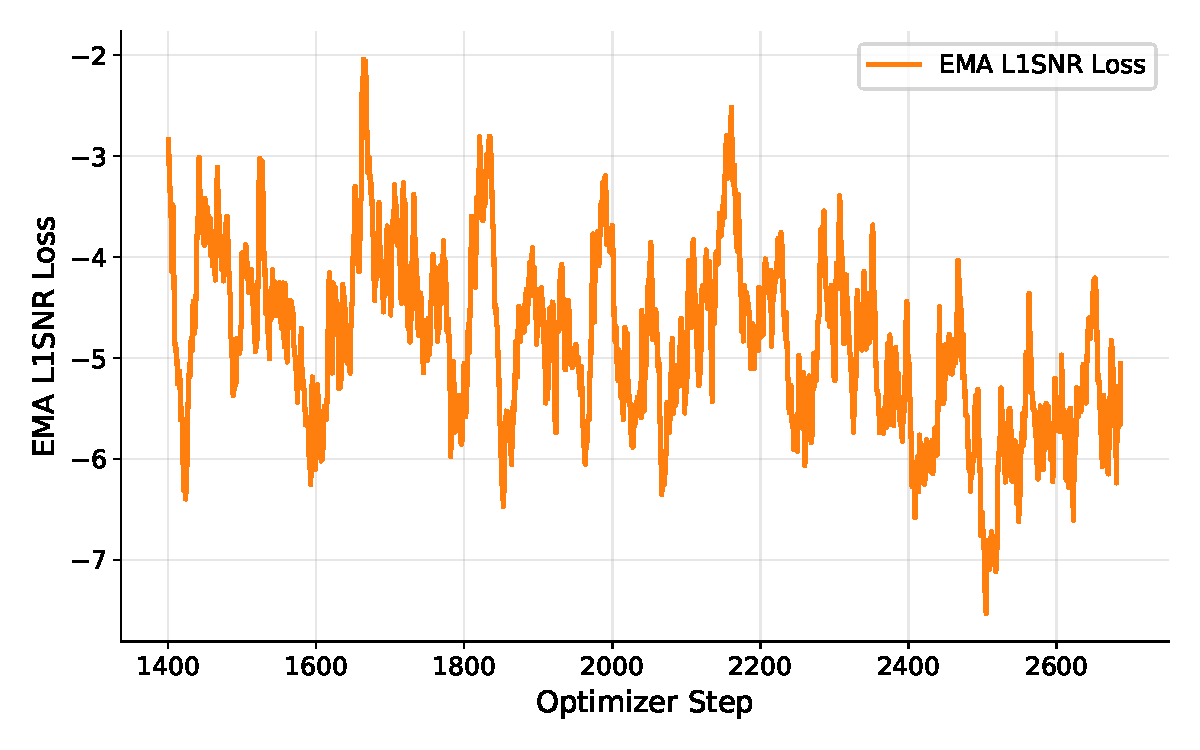
\includegraphics[width=0.8\linewidth]{paper_figures/run002_training_trajectory.pdf}
    \caption{Training trajectory of the Exponential Moving Average (EMA) of the L1SNR training objective across global optimizer steps during Run 002.}
    \label{fig:training_trajectory}
\end{figure}

\begin{figure}[t]
    \centering
    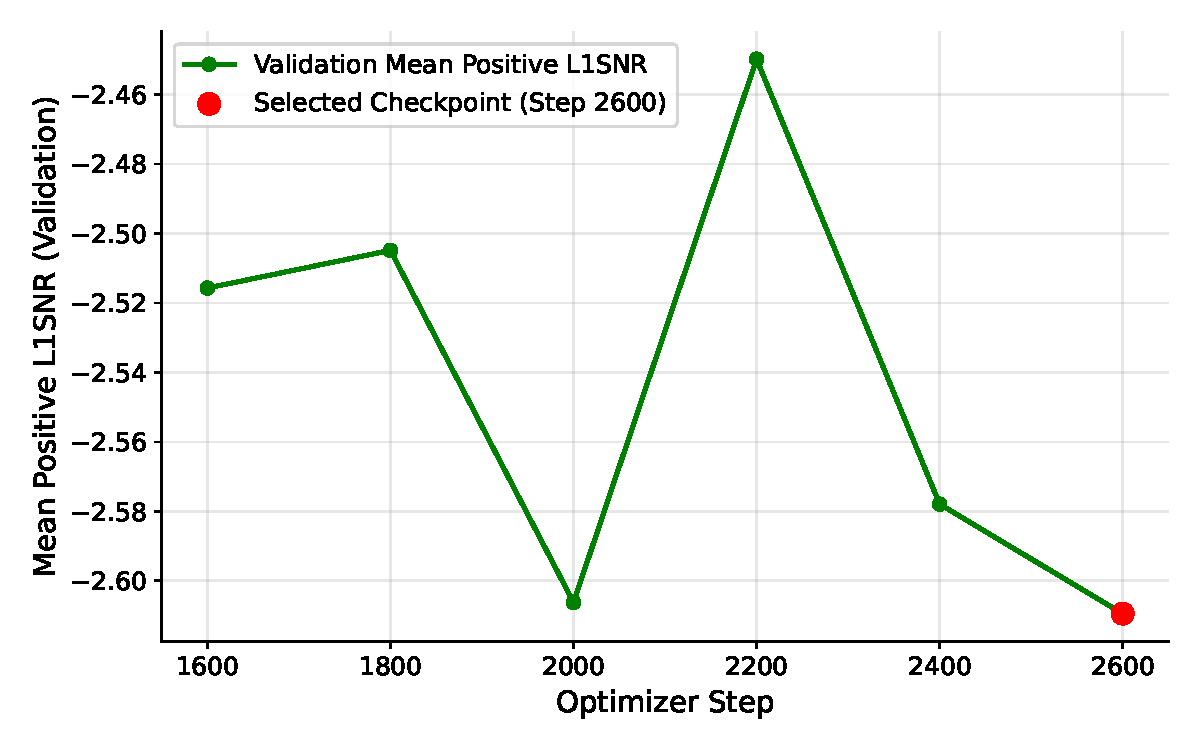
\includegraphics[width=0.8\linewidth]{paper_figures/run002_validation_trajectory.pdf}
    \caption{Validation trajectory of mean positive L1SNR across evaluation checkpoints during Run 002. Checkpoint selection was based on this validation objective subject to the predefined negative-query RMS safety condition.}
    \label{fig:validation_trajectory}
\end{figure}
